\chapter{Programmierung mit Rust und Unterschiede zu C/C++}

In diesem Kapitel wird die Programmierung mit Rust gezeigt, dabei werden auch einige Unterschiede zu C und C++ erläutert.


\section{Grundlagen}

Zu den Grundlagen einer jeden Programmiersprache gehört der Umgang mit Variablen und Datentypen. Kontrollstrukturen definieren dabei die Reihenfolge, in der Berechnungen durchgeführt werden.

\subsection{Variablen und Mutabilität}

In Rust sind Variablen standardmäßig unveränderlich. Das ist einer von vielen Faktoren, die Programmierer helfen sollen, Fehler im Code besser auffinden zu können. \cite{RustBook}

Ein Beispiel in Rust:

\begin{lstlisting}
    fn main() {
        let x = 5;
        println!("The value of x is {}", x);
        x = 6;
        println!("The value of x is {}", x);
    }
\end{lstlisting}

Beim Kompilieren erscheint folgende Fehlermeldung:

\begin{lstlisting}
    error[E0384]: cannot assign twice to immutable variable 
    `x`
    --> src/main.rs:4:5
     |
   2 |     let x = 5;
     |         -
     |         |
     |         first assignment to `x`
     |         help: make this binding mutable: `mut x`
   3 |     println!("The value of x is {}", x);
   4 |     x = 6;
     |     ^^^^^ cannot assign twice to immutable variable
   
\end{lstlisting}

Die Fehlermeldung besagt, dass ein unveränderlicher Wert nicht verändert werden darf, und schlägt vor, den Wert veränderlich, also als \glqq mutable\grqq{}, zu deklarieren.

In C oder C++ ist jede Variablendefinition standardmäßig veränderlich, das heißt bei gleicher Vorangehensweise würde folgendes C-Programm fehlerfrei übersetzen:

\begin{lstlisting}
    #include <stdio.h>

    int main()
    {
        int x = 5;
        printf("The value of x is %d\n", x);
        x = 6;
        printf("The value of x is %d\n", x);
        return 0;
    }    
\end{lstlisting}

Das Schlüsselwort \verb"const" kann verwendet werden, um Werte in C/C++ konstant zu deklarieren.

\begin{lstlisting}
    const int x = 5;
\end{lstlisting}

Wird aber beispielsweise in C versucht, ein konstant deklarierter Wert zu ver\-än\-dern, indem eine Variable mit einem nicht konstanten Typ verwendet wird, ist das Verhalten nicht definiert. \cite[p.~87]{ISO:9899:2017}

Das Verhalten in folgendem Beispielprogramm ist somit nicht definiert und kann von vielen verschiedenen Faktoren abhängen:

\begin{lstlisting}
    #include <stdio.h>

    int main()
    {
        const int x = 5;
        printf("The value of x is %d\n", x);
        *(int *)&x = 6;
        printf("The value of x is %d\n", x);
        return 0;
    }
\end{lstlisting}

Ergebnis mit dem Clang Compiler in der Version 7.0.1 auf einem Linux System (keine Warnungen beim Kompilieren):

\begin{lstlisting}
    The value of x is 5
    The value of x is 5
\end{lstlisting}

Ergebnis mit dem GCC Compiler in der Version 8.3.1 auf einem Linux System (auch hier keine Warnungen):

\begin{lstlisting}
    The value of x is 5
    The value of x is 6
\end{lstlisting}

\subsection{Datentypen}\label{chap:datatypes}

Jede Variable in Rust hat einen bestimmten Datentyp. In Rust wird unterschieden zwischen skalaren und zusammengesetzten Typen. Rust ist eine statisch typisierte Sprache, somit müssen die Typen aller Variablen zur Kompilierzeit bekannt sein. Der Compiler kann normalerweise ableiten, welcher Typ verwenden soll basierend auf dem Wert und wie er verwendet wird. In Fällen, in denen viele Typen möglich sind, z. B. wenn ein String in einen numerischen Typ konvertiert werden soll, muss eine Typannotation hinzugefügt werden:

\begin{lstlisting}
    let guess: u32 = "42".parse().expect("Not a number!");
\end{lstlisting}

Ohne Angabe des Typs würde der Rust-Compiler eine Fehlermeldung ausgeben.

\subsubsection{Integer Typ}

Ein Integer ist ein Datentyp für ganze Zahlen. Der Typ \verb"u32" gibt an, dass es sich um eine vorzeichenlose Ganzzahl handelt. Vorzeichenbehaftete Ganzzahltypen beginnen mit \glqq i\grqq{} an Stelle von \glqq u\grqq{} und die Zahl gibt an, wie viel Speicherplatz sie beansprucht. Folgende Tabelle zeigt die Integertypen von Rust und C:

\begin{table}[htbp]
\centering
\begin{tabular}{|c||c|c||c|c|}
\hline
\rule[-1ex]{0pt}{2.5ex} & \multicolumn{2}{|c||}{Rust} & \multicolumn{2}{|c|}{C/C++} \\
\hline
\rule[-1ex]{0pt}{2.5ex} Länge & signed & unsigned & signed & unsigned \\
\hline
\rule[-1ex]{0pt}{2.5ex} 8-bit & i8 & u8 & \_\_int8\_t & \_\_uint8\_t \\
\hline
\rule[-1ex]{0pt}{2.5ex} 16-bit & i16 & u16 & \_\_int16\_t & \_\_uint16\_t \\
\hline
\rule[-1ex]{0pt}{2.5ex} 32-bit & i32 & u32 & \_\_int32\_t & \_\_uint32\_t \\
\hline
\rule[-1ex]{0pt}{2.5ex} 64-bit & i64 & u64 & \_\_int64\_t & \_\_uint64\_t \\
\hline
\rule[-1ex]{0pt}{2.5ex} 128-bit & i128 & u128 & \_\_int128\_t & \_\_uint128\_t \\
\hline
\rule[-1ex]{0pt}{2.5ex} arch & isize & usize & & \\
\hline
\end{tabular}
\caption{Integertypen in Rust und C/C++}
\end{table}

In C sollen mit \verb"short" und \verb"long" verschieden lange ganzzahlige Werte zur Ver\-fü\-gung stehen, soweit dies praktikabel ist; \verb"int" wird normalerweise die natürliche Größe für eine bestimmte Maschine sein. \verb"short" belegt oft 16 Bits, \verb"long" 32 Bits und \verb"int" entweder 16 oder 32 Bits. Es steht jedem Übersetzer frei, sinnvolle Größen für seine Maschine zu wählen, nur mit den Einschränkungen, dass \verb"short" und \verb"int" wenigstens 16 Bits haben, \verb"long" mindestens 32 Bits, und dass \verb"short" nicht länger als \verb"int" und \verb"int" nicht länger als \verb"long" sein darf. \cite{ProgInC}

Beispiel:

\begin{lstlisting}
    printf("%zu\n", sizeof(char));      // 1:  8-bit
    printf("%zu\n", sizeof(short));     // 2: 16-bit
    printf("%zu\n", sizeof(int));       // 4: 32-bit
    printf("%zu\n", sizeof(long));      // 8: 64-bit
\end{lstlisting}

In Rust hängen die Typen \verb"isize" und \verb"usize" von der Art des Computers ab, auf dem das Programm ausgeführt wird: 64 Bits bei 64-Bit-Architekturen und 32 Bits bei 32-Bit-Architekturen.

In Rust wird standardmäßig der Integertyp i32 verwendet. Dieser Typ ist im Allgemeinen der schnellste Typ, auch auf 64-Bit-Systemen. Die Typen \verb"isize" und \verb"usize" können zum Indexieren von Arrays verwendet werden.

\subsubsection{Weitere Typen in Rust}

\begin{itemize}
    \item Fließkomma-Typen: \verb"f32" und \verb"f64" (Standard ist \verb"f64")
    \item Boolean: \verb"bool" true / false
    \item Zeichentyp \verb"char": Unicode, das heißt chinesische, japanische und koreanische Zeichen, Emoji, Leerzeichen mit Nullbreite sind möglich
\end{itemize}

\subsubsection{Tupel}

Ein Tupel ist ein allgemeiner Weg, um einige andere Werte mit verschiedenen Typen zu einem Verbindungstyp zu gruppieren. Tupel haben eine feste Länge und können somit nicht größer oder kleiner werden nachdem sie deklariert wurden.

\begin{lstlisting}
    fn main() {
        let tup: (i32, f64, u8) = (500, 6.4, 1);
        let (x, y, z) = tup;
        println!("The value of y is: {}", y);
        println!("The value of z is: {}", tup.2);
    }
\end{lstlisting}

\subsubsection{Arrays}

Eine andere Möglichkeit, Sammlungen mehrerer Werte zu bilden, sind Arrays. Im Gegensatz zu einem Tupel muss jedes Element eines Arrays denselben Typ haben. Arrays in Rust unterscheiden sich von Arrays in einigen anderen Sprachen, da Arrays in Rust eine feste Länge haben.

In Rust werden die Werte, die direkt in ein Array gespeichert werden sollen, als eine durch Kommata getrennte Liste in eckigen Klammern geschrieben:

\begin{lstlisting}
    let a = [1, 2, 3, 4, 5];
\end{lstlisting}

Arrays sind nützlich, um Daten auf dem Stack statt auf dem Heap zuweisen zu können oder um sicherzustellen, dass immer eine feste Anzahl von Elementen vorhanden sind. Ein Array ist jedoch nicht so flexibel wie der Vektortyp. Ein Vektor ist ein ähnlicher Auflistungstyp, der von der Standardbibliothek bereitgestellt wird und dessen Größe dynamisch verändert werden kann.

Die Schreibweise des Array-Typs erfolgt mit eckigen Klammern mit dem Typen der Elemente gefolgt von einem Semikolon und die Anzahl der Elemente für das Array:

\begin{lstlisting}
    let a: [i32; 5] = [1, 2, 3, 4, 5];
\end{lstlisting}

Eine ähnliche Schreibweise wird zum Initialisieren eines Arrays verwendet, das für jedes Element den selben Wert enthält. Dabei wird der Anfangswert, dann ein Semikolon und die Länge des Arrays angegeben:

\begin{lstlisting}
    let a = [3; 5];
\end{lstlisting}

Das Array \verb"a" enthält 5 Elemente, die zunächst alle auf den Wert 3 gesetzt wurden. Folgender Ausdruck erzeugt das gleiche Array:

\begin{lstlisting}
    let a = [3, 3, 3, 3, 3];
\end{lstlisting}

Ein Array ist ein einzelner Speicherbereich, der auf dem Stack reserviert ist. Es kann mithilfe eines Indexes auf die Elemente zugegriffen werden:

\begin{lstlisting}
    let a = [1, 2, 3, 4, 5];
    let first = a[0];
    let second = a[1];
\end{lstlisting}

Wird auf ein Element zugegriffen, das außerhalb des Bereichs ist, beendet sich das Programm mit folgender Meldung:

\begin{lstlisting}
    thread 'main' panicked at 'index out of bounds: the len
    is 5 but the index is 10', src/main.rs:5:13
    note: Run with `RUST_BACKTRACE=1` environment variable
    to display a backtrace.
\end{lstlisting}

Wenn in C oder C++ auf ein Element außerhalb des Bereichs eines Arrays zugegriffen wird, fällt dies beim Testen wesentlich weniger auf, da normalerweise das Programm weiter ausgeführt wird.

Das ist ein Beispiel der Sicherheitsprinzipien von Rust. Viele Low-Level-Pro\-gram\-mier\-spra\-chen verzichten auf diesen Check, sodass ein ungültiger Speicherbereich indexiert werden kann. Rust verhindert dies durch sofortiges Beenden des Programms.

\subsection{Funktionen}

In Rust werden Funktionen und Variablennamen als Konvention in snake case geschrieben. Ein Programm, das eine Beispielfunktion enthält könnte so aussehen:

\begin{lstlisting}
    fn main() {
        println!("Hello, world!");
        another_function(42);
    }
    fn another_function(n: i32) {
        println!("Another function with number {}.", n);
    }
\end{lstlisting}

Eine Funktion mit Parameter enthält den Namen der Variable sowie den Typen mit einem Doppelpunkt getrennt. Bei mehreren Parametern werden diese mit Komma getrennt.

Bei Funktionen mit Rückgabewerten kann am Ende des Funktionskörpers der Rückgabewert als Expression ohne Semikolon geschrieben werden. Wenn eine Funktion früh beendet werden soll, kann ein \verb"return" mit Rückgabewert benutzt werden. Der Rückgabetyp der Funktion muss mit einem Pfeil (\verb"->") geschrieben werden.

\begin{lstlisting}
    fn main() {
        let result = add(12, 34);
        println!("The result is {}.", result);
    }
    fn add(n1: i32, n2: i32) -> i32 {
        n1 + n2
    }
\end{lstlisting}

\subsection{Kontrollstrukturen}

Kontrollstrukturen definieren die Reihenfolge, in der Berechnungen durchgeführt werden. Die Entscheidung, ob Code ausgeführt werden soll oder nicht, abhängig davon, ob eine Bedingung wahr ist, und die Entscheidung, wiederholt Code aus\-zu\-füh\-ren, während eine Bedingung wahr ist, sind grundlegende Bausteine in den meisten Programmiersprachen. Die häufigsten Konstrukte, mit denen der Ausführungsfluss von Rust-Code gesteuert werden können, sind \verb"if"-Ausdrücke und Schleifen.

\subsubsection{\texttt{if}-Anweisungen}

Mit \verb"if"-\verb"else"-Anweisungen werden Entscheidungen formuliert. Der \verb"else"-Teil ist optional.

Beispiel:

\begin{lstlisting}
    if number < 5 {
        println!("condition was true");
    } else {
        println!("condition was false");
    }
\end{lstlisting}

Diese Anweisungen sind syntaktisch wie C oder C++, mit dem Unterschied, dass keine Klammern bei der Expression benötigt wird.

In Rust muss der Typ der Expression ein Boolean sein. Folgendes Programm wird also nicht übersetzt:

\begin{lstlisting}
    fn main() {
        let number = 3;
        if number {                     // type must be bool
            println!("number was three");
        }
    }
\end{lstlisting}

C und C++ prüfen bei einer \verb"if"-Anweisung mit einem Integer Wert nur, ob dieser den Wert 0 hat. Da in Rust ein Boolean Typ benötigt wird, muss das obige Programm umgeschrieben werden:

\begin{lstlisting}
    fn main() {
        let number = 3;
        if number != 0 {
            println!("number was something other than 0");
        }
    }
\end{lstlisting}

Mehrere Bedingungen können auch in Rust in einer \verb"else if"-Anweisung behandelt werden:

\begin{lstlisting}
    let number = 6;

    if number % 4 == 0 {
        println!("number is divisible by 4");
    } else if number % 3 == 0 {
        println!("number is divisible by 3");
    } else if number % 2 == 0 {
        println!("number is divisible by 2");
    } else {
        println!("number is not divisible by 4, 3, or 2");
    }
\end{lstlisting}

In Rust kann die \verb"if"-Anweisung eine Expression verpacken um z. B. Werte von Variablen zu definieren, ähnlich wie der \verb"?:"-Operator in C/C++:

\begin{lstlisting}
    let condition = true;
    let number = if condition {
        5
    } else {
        6
    };
\end{lstlisting}

Da Rust eine statisch typisierte Sprache ist, muss der Typ beim Kompilieren bekannt sein. Das bedeutet, dass bei dieser \verb"if"-Anweisung der Typ einheitlich sein muss. Im letzten Beispiel ist \verb"number" vom Typ \verb"i32".

\subsubsection{Schleifen}

Rust hat drei Arten von Schleifen: loop, while und for.

Loop-Schleifen führen Code so oft aus, bis sie explizit mit dem Schlüsselwort \verb"break" gestoppt werden. Schleifen können in Rust auch als Expression verwendet werden wenn an dem \verb"break" eine Expression angefügt wird:

\begin{lstlisting}
    fn main() {
        let mut counter = 0;
        let result = loop {
            counter += 1;
            if counter == 10 {
                break counter * 2;      // loop returning 20
            }
        };
        println!("The result is {}", result);
    }
\end{lstlisting}

\verb"while"-Schleifen gibt es auch in C und C++. In Rust ist die Syntax ähnlich:

\begin{lstlisting}
    fn main() {
        let a = [10, 20, 30, 40, 50];
        let mut index = 0;
        while index < 5 {
            println!("the value is: {}", a[index]);
            index = index + 1;
        }
    }
\end{lstlisting}

Das Programm gibt alle Werte aus dem Array aus. Alternativ kann hier mit einer \verb"for"-Schleife gearbeitet werden. For-Schleifen funktionieren in Rust anders als in C oder C++, sie gleichen ehr einer \verb"for"-\verb"each"-Schleife aus Java. Das bedeutet, dass der Code innerhalb der Schleife für jedes Element aus einer Sammlung einmal ausgeführt wird.

\begin{lstlisting}
    fn main() {
        let a = [10, 20, 30, 40, 50];
        for element in a.iter() {
            println!("the value is: {}", element);
        }
    }
\end{lstlisting}

Mit \verb"for"-Schleifen kann in Rust die Stabilität des Programms erhöht werden, da Zugriffe außerhalb eines Arrays verhindert werden können.


\section{Ownership}

Ownership ist ein einzigartiges Merkmal von Rust. Es ermöglicht Speichersicherheit zur Kompilierzeit ohne die Notwendigkeit eines Garbage Collectors. Daher ist es wichtig, das Ownership-Prinzip als Programmierer zu verstehen. In diesem Kapitel werden Ownership und damit zusammenhängende Eigenschaften wie Borrowing, Slices und wie Rust Daten im Arbeitsspeicher ablegt, beschrieben.

\subsection{Funktionsweise von Ownership}

Alle Computerprogramme müssen Arbeitsspeichermanagement betreiben. Man\-che Sprachen benutzen einen Garbage Collector, welcher während der Programmlaufzeit nach nicht mehr verwendeten Speicher sucht und diesen anschließend frei gibt. In andern Sprachen muss der Programmierer explizit Speicher zuweisen und freigeben. Rust geht anders vor: Speicher wird durch ein System von Besitz und einen Satz an Regeln gestützt, welches der Compiler zur Kompilierzeit überprüft, sodass das Programm zur Laufzeit nicht gebremst wird.

\subsubsection{Regeln}

\begin{itemize}
    \item Jeder Wert in Rust hat eine Variable, die als Eigentümer bezeichnet wird.
    \item Es gibt für jeden Wert nur einen aktiven Eigentümer.
    \item Wenn der Besitzer den Gültigkeitsbereich verlässt, wird der Wert gelöscht.
\end{itemize}

\subsubsection{Beispiel: String}

Um die Eigentumsregeln zu veranschaulichen, ist ein komplexerer Datentyp not\-wen\-dig als die, die in \autoref{chap:datatypes} behandelt wurden, denn diese werden auf dem Stack gespeichert. In diesem Beispiel sollen Daten, die auf dem Heap gespeichert werden, betrachtet werden um zu veranschaulichen, wie Rust erkennt, wann diese Daten zu bereinigen sind. Hierfür wird im Folgenden der Typ \verb"String" verwendet. Diese Aspekte gelten auch für andere komplexe Datentypen, die von der Standardbibliothek bereitgestellt werden.

Wenn ein Rust-Programm eine Eingabe von einem Benutzer speichern möchte, muss ein Datentyp verwendet werden, welche eine variable Länge haben kann. Einen solchen String kann man in Rust zum Beispiel mit der \verb"from"-Funktion erstellen:

\begin{lstlisting}
    let mut s = String::from("hello");
    s.push_str(", world!");             // appends a literal
    println!("{}", s);                  // 'hello, world!'
\end{lstlisting}

Um einen veränderlichen String zu erzeugen, muss Speicherplatz auf dem Heap zugewiesen werden, dessen größe zur Kompilierzeit unbekannt ist. Das heißt:

\begin{enumerate}
    \item Speicherplatz muss vom Betriebssystem zur Laufzeit bereitgestellt werden und
    \item der Speicherplatz muss wieder freigegeben werden, wenn der String nicht mehr benötigt wird.
\end{enumerate}

Der erste Teil wird manuell vom Programmierer beim Aufruf von \verb"String::from" initiiert. Der zweite Teil geschieht automatisch intern durch die Methode \verb"drop", sobald der Besitzer den Gültigkeitsbereich verlässt, zum Beispiel am Ende eines Blocks.

\begin{lstlisting}
    {
        let s = String::from("hello");
        // s is valid from this point forward
    
        // doo stuff with s
    }                    // this scope is now over, and s is
                         // no longer valid
\end{lstlisting}

In C++ wird dieses Muster der Freigabe von Ressourcen am Ende der Lebensdauer eines Elements manchmal als \textit{Ressourcenbelegung ist Initialisierung (Resource Acquisition Is Initialization, kurz RAII)} bezeichnet. \cite[p.~71]{CppProg}

Dieses Muster hat einen tiefgründigen Einfluss auf die Schreibweise von Rust-Code. Es mag einfach erscheinen, aber das Verhalten von Code kann in komplizierten Situationen unerwartet sein, wenn mehrere Variablen die Daten verwenden sollen, die auf dem Heap zugewiesen wurden.

\subsubsection{Variablen und Daten: Move}

Mehrere Variablen können in Rust auf unterschiedliche Weise mit denselben Daten interagieren. Ein Beispiel mit Integer:

\begin{lstlisting}
    let x = 5;
    let y = x;
\end{lstlisting}

Hier wird der Wert 5 an die Konstante \verb"x" gebunden und anschließend eine Kopie von \verb"x" an die Konstante \verb"y" gebunden. Der Wert wird hier kopiert, da Integer eine feste Größe im Speicher haben und auf dem Stack gespeichert werden.

Beispiel mit String:

\begin{lstlisting}
    let s1 = String::from("hello");
    let s2 = s1;
\end{lstlisting}

Dies sieht dem vorherigen Code sehr ähnlich, aber die Funktionsweise ist nicht dieselbe, denn Strings werden in Rust im Heap gespeichert.

\begin{figure}[htbp]
    \centering
    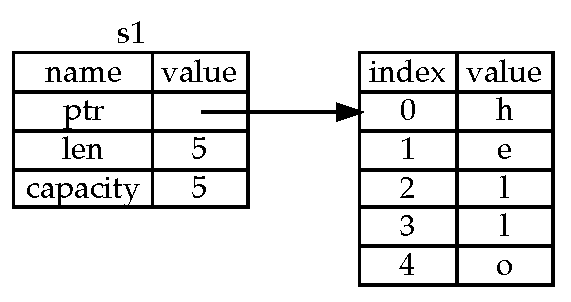
\includegraphics[scale=0.9]{Programmierung/Tabelle1.pdf}
    \caption{Repräsentation des Speichers eines String}
    \label{fig:tabelle1}
\end{figure}

\autoref{fig:tabelle1} zeigt die Bestandteile eines String. Er besteht aus drei Teilen, zu sehen in der linken Tabelle: ein Pointer auf den Speicher, der den String enthält, die Länge und die Kapazität. Diese Datengruppe wird auf dem Stack gespeichert. In der rechten Tabelle ist sich der Speicher auf dem Heap dargestellt.

Bei der Zuweisung von \verb"s1" zu \verb"s2" werden nur die String-Daten kopiert, das heißt der Pointer, die Länge und die Kapazität, welche sich auf dem Stack befinden. Die Daten des Heaps werden nicht kopiert.

\begin{figure}[htbp]
    \centering
    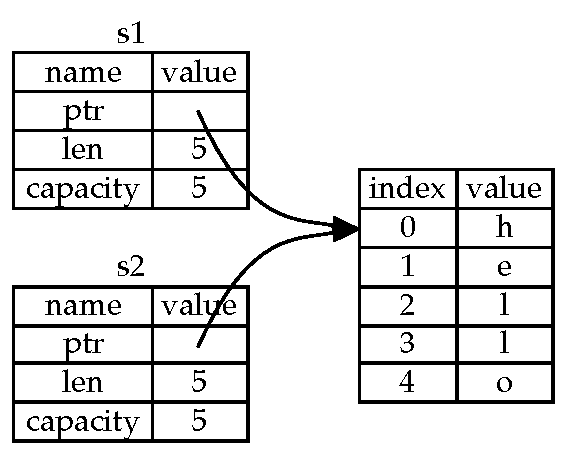
\includegraphics[scale=0.9]{Programmierung/Tabelle2.pdf}
    \caption{Repräsentation des Speichers eines String: Kopie auf dem Stack}
    \label{fig:tabelle2}
\end{figure}

Wenn Rust eine vollständige Kopie gemacht hätte, würden die Daten wie auf \autoref{fig:tabelle3} aussehen und die Operation \verb"s2 = s1" wäre hinsichtlich der Lauf\-zeit\-leis\-tung sehr teuer.

\begin{figure}[htbp]
    \centering
    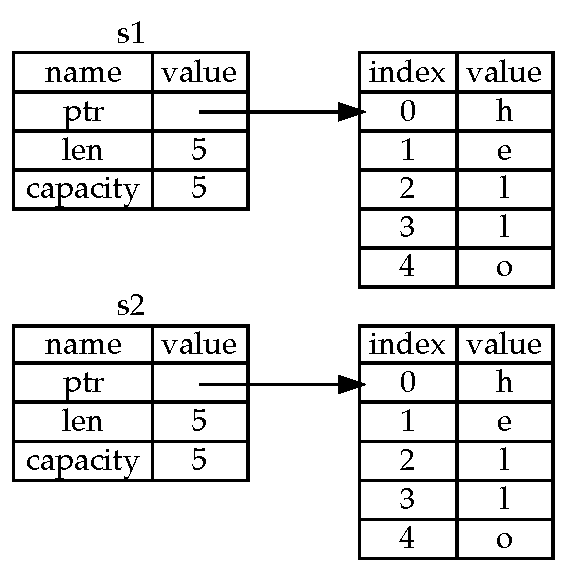
\includegraphics[scale=0.9]{Programmierung/Tabelle3.pdf}
    \caption{Repräsentation des Speichers eines String: Vollständige Kopie}
    \label{fig:tabelle3}
\end{figure}

Sobald eine Variable außerhalb des Gültigkeitsbereichs gelangt, wird der Spei\-cher aus dem Heap gelöscht. Aber da \autoref{fig:tabelle2} zwei Variablen zeigt, die auf den selben Speicherbereich im Heap zeigen, würde zwei mal der Speicherbereich freigegeben werden. Das ist bekannt als \glqq double free\grqq{}-Error und kann zu Speicherbeschädigungen und möglicherweise zu Sicherheitsanfälligkeiten führen.

Um die Speichersicherheit zu gewährleisten, hält Rust \verb"s1" für ungültig und muss somit nichts löschen, wenn \verb"s1" den Gültigkeitsbereich verlässt.

Das hat zu Folge, dass \verb"s1" nicht mehr genutzt werden kann, nachdem es \verb"s2" zugewiesen wurde:

\begin{lstlisting}
    let s1 = String::From("hello");
    let s2 = s1;

    println!("{}, world!", s1);         // error
\end{lstlisting}

Daraus entsteht folgende Fehlermeldung:


\begin{lstlisting}
    error[E0382]: borrow of moved value: `s1`
     --> src/main.rs:5:28
      |
    3 |     let s1 = String::from("hello");
      |         -- move occurs because `s1` has type
    `std::string::String`, which does not implement the
    `Copy` trait
    4 |     let s2 = s1;
      |              -- value moved here
    5 |     println!("{}, world!", s1);
      |                            ^^ value borrowed here
    after move
\end{lstlisting}

Diese Art von Kopieren, welche die erste Variable ungültig macht, wird in Rust \glqq move\grqq{} genannt (\verb"s1" was \textit{moved} into \verb"s2"). Was also tatsächlich passiert, wird in \autoref{fig:tabelle4} dargestellt.

\begin{figure}[htbp]
    \centering
    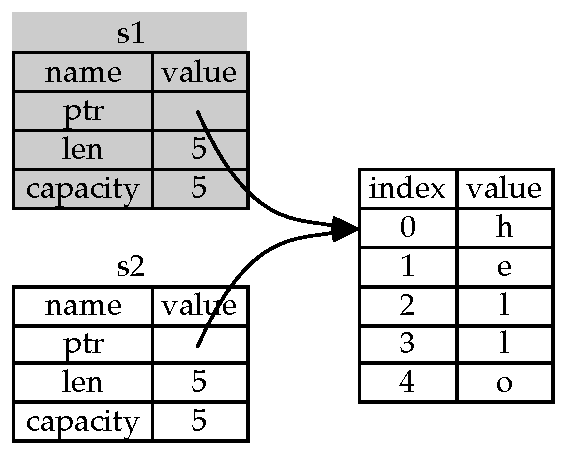
\includegraphics[scale=0.9]{Programmierung/Tabelle4.pdf}
    \caption{Repräsentation des Speichers eines String: Moved}
    \label{fig:tabelle4}
\end{figure}

Folglich gibt es in Rust keine \glqq double free\grqq{}-Error, da der Speicher nur einmal freigegeben wird, nämlich wenn \verb"s2" den Gültigkeitsbereich verlässt.

\subsubsection{Variablen und Daten: Clone}

Wenn eine vollständige Kopie erstellt werden soll, kann die Methode \verb"clone" benutzt werden:

\begin{lstlisting}
    let s1 = String::from("hello");
    let s2 = s1.clone();

    println!("s1 = {}, s2 = {}", s1, s2);
\end{lstlisting}

Der Code kompiliert ohne Fehlermeldungen und erzeugt explizit das in \autoref{fig:tabelle3} gezeigte Verhalten, bei dem auch die Heap-Daten kopiert werden.

\subsubsection{Stack-Only-Daten kopieren}

Primitive Datentypen, die komplett auf dem Stack gespeichert sind, können nicht übergeben werden (Move nicht möglich), sie können nur vollständig kopiert werden. Darum würde folgender Code ohne Fehler übersetzen:

\begin{lstlisting}
    let x = 5;
    let y = x;

    println!("x = {}, y = {}", x, y);
\end{lstlisting}

Integer besitzen eine feste Speichergröße zur Kompilierzeit und es macht keinen Unterschied, sie mit \verb"clone" zu kopieren. Wenn ein Typ den \verb"Copy"-Trait besitzt, kann die erste Variable nach der Zuweisung weiter verwendet werden. In der Regel kann jede Gruppe einfacher Skalarwerte über den Stack vollständig kopiert werden. Einige der Typen sind:

\begin{itemize}
    \item Alle Integer-Typen, z. B. \verb"u32"
    \item Boolean-Typ, \verb"bool" mit den Werten \verb"true" und \verb"false"
    \item Alle Fließkommazahlen wie z. B. \verb"f64"
    \item Zeichentyp \verb"char"
    \item Tupel, wenn sie nur Typen beinhalten, die den \verb"Copy"-Trait implementieren z. B. \verb"(i32, i32)", jedoch nicht \verb"(i32, String)"
\end{itemize}

\subsubsection{Ownership und Funktionen}

Die Semantik für die Übergabe eines Wertes an eine Funktion ähnelt derjenigen, die einer Variablen einen Wert zuweist. Beim Übergeben einer Variablen an eine Funktion wird genauso wie bei einer Zuweisung verschoben oder kopiert. Folgendes Programm enthält ein Beispiel mit einigen Anmerkungen, wann Variablen in den Geltungsbereich gelangen und wieder herauskommen:

\begin{lstlisting}
    fn main() {
        let s = String::from("hello");  // s comes
                                        // into scope
        takes_ownership(s);         // s's value moved into
                                    // the function...
        // ... and is no longer valid here

        let x = 5;         // x comes into scope

        makes_copy(x);     // x would move into the function
                           // but i32 is Copy, so it's okay
                           // to still use x afterward

    } // Here, x goes out of scope, then s. But because s's
      // value was moved, nothing special happens.


    fn takes_ownership(some_string: String) {
        // some_string comes into scope

        println!("{}", some_string);
    } // Here, some_string goes out of scope and 'drop' is
      // called. The backing memory is freed.


    fn makes_copy(some_integer: i32) {
        // some_integer comes into scope

        println!("{}", some_integer);
    } // Here, some_integer goes out of scope. Nothing
      // special happens.
\end{lstlisting}

Wenn \verb"s" nach der Methode \verb"takes_ownership" genutzt wird, würde Rust einen Fehler bei der Kompilierung ausgeben. Diese statischen Checks sollen Fehler im Programm verhindern.

Funktionen können Ownership durch einen Rückgabewert auch wieder zu\-rück\-ge\-ben:

\begin{lstlisting}
    fn main() {
        let s1 = gives_ownership();
        let s2 = takes_and_gives_back(s1);
        println!("{}, world!", s1); // error
        println!("{}, world!", s2); // this works
    }

    fn gives_ownership() -> String {
        let some_string = String::from("hello");
        some_string
    }

    fn takes_and_gives_back(a_string: String) -> String {
        a_string
    }
\end{lstlisting}

\subsection{Referenzen und Borrowing}

Eine Funktion, welche die Länge eines String berechnet und die Ownership des verwendeten Strings wieder zurückgibt, könnte so aussehen:

\begin{lstlisting}
    fn main() {
        let s1 = String::from("hello");
        let (s2, len) = calculate_length(s1);
        println!("The length of '{}' is {}.", s2, len);
    }
    fn calculate_length(s: String) -> (String, usize) {
        let length = s.len();
        (s, length)
    }
\end{lstlisting}

Dies ist jedoch viel Aufwand für ein Konzept, das gebräuchlich sein sollte. Daher können in Rust Referenzen verwendet werden.

So wird die \verb"calculate_length" Funktion definiert und benutzt, die eine Referenz auf ein Objekt als Parameter enthält, anstatt die Ownership zu übernehmen:

\begin{lstlisting}
    fn main() {
        let s1 = String::from("hello");
        let len = calculate_length(&s1);
        println!("The length of '{}' is {}.", s1, len);
    }
    fn calculate_length(s: &String) -> usize {
        s.len()
    }
\end{lstlisting}

Der gesamte Tupelcode in der Variablendeklaration und der Funk\-ti\-ons\-rück\-ga\-be\-wert ist weg. Außerdem wird \verb"&s1" in \verb"calculate_length" und in seiner Definition \verb"&String" anstelle von \verb"String" benutzt.

Die \verb"&"-Zeichen erstellen Referenzen und ermöglichen auf einen bestimmten Wert zu verweisen, ohne dessen Ownership zu beanspruchen. \autoref{fig:tabelle5} zeigt ein Diagramm hierzu.

\begin{figure}[htbp]
    \centering
    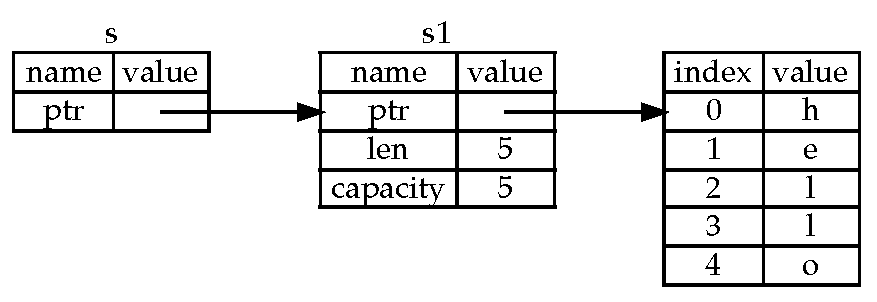
\includegraphics[scale=0.9]{Programmierung/Tabelle5.pdf}
    \caption{Diagramm von \texttt{\&String} \texttt{s} Zeiger auf \texttt{String} \texttt{s1}}
    \label{fig:tabelle5}
\end{figure}

Mit der \verb"&s1" Syntax kann eine Referenz erstellt werden, die sich auf den Wert von \verb"s1" bezieht, ihm aber nicht gehört. Der Wert auf den er verweist wird nicht gelöscht, wenn die Referenz den Gültigkeitsbereich verlässt.

Ebenso verwendet die Signatur der Funktion \verb"&" um anzuzeigen, dass der Typ des Parameters eine Referenz ist.

Das Gegenteil der Referenzierung mit \verb"&" ist die Dereferenzierung, die mit dem Dereferenzierungsoperator \verb"*" erzielt wird.

Der Gültigkeitsbereich von \verb"s" ist der eines normalen Funktionsparameters, jedoch wird der Wert nicht aus dem Speicher gelöscht, da keine Ownership an \verb"s" übergeben wurde, weshalb auch keine zurückgegeben werden muss. Referenzen als Funktionsparameter werden in Rust \glqq Borrowing\grqq{} genannt. Wie in der realen Welt kann Eigentum an andere ausgeliehen werden und wenn die andere Person es nicht mehr braucht, kann diese es wieder an den Eigentümer zurückgeben.

Genauso wie Variablen standardmäßig unveränderlich sind, gilt dies auch für Referenzen. Es kann nichts verändert werden, auf das nur mit \verb"&" referenziert wird. Folgender Code würde daher nicht funktionieren:

\begin{lstlisting}
    fn main() {
        let s = String::from("hello");
        change(&s);
    }
    fn change(some_string: &String) {
        some_string.push_str(", world"); // error
    }
\end{lstlisting}

\subsubsection{Veränderbare Referenzen}

Kleine Veränderungen beheben den Fehler aus dem obigen Programm:

\begin{lstlisting}
    fn main() {
        let mut s = String::from("hello");
        change(&mut s);
    }
    fn change(some_string: &mut String) {
        some_string.push_str(", world"); // works now
    }
\end{lstlisting}

Die Variable \verb"s" muss veränderbar gemacht werden durch Kennzeichnung mit \verb"mut". Es wird nun eine veränderbare Referenz übergeben und die Funktion erwartet nun auch eine entsprechende Referenz mit \verb"some_string: &mut String".

Veränderbare Referenzen haben eine große Einschränkung: Es darf nur eine veränderbare Referenz auf ein bestimmtes Datenelement in einem bestimmeten Bereich aktiv sein. Folgender Code würde somit nicht kompilieren:

\begin{lstlisting}
    let mut s = String::from("hello");
    let r1 = &mut s;
    let r2 = &mut s;                    // error
    println!("{}, {}", r1, r2);
\end{lstlisting}

Diese Einschränkung erlaubt kontrollierte Verwendung von Variablen. Mithilfe dieser Regel verhindert Rust sogenannte \glqq data races\grqq{}. Diese ähneln \glqq race conditions\grqq{} und treten auf, wenn drei Verhaltensweisen auftreten:

\begin{itemize}
    \item Zwei oder mehr Pointer greifen zeitgleich auf den selben Speicherbereich zu.
    \item Mindestens einer der Pointer schreiben.
    \item Kein Mechanismus wird verwendet, um den Zugriff der Daten zu synchronisieren.
\end{itemize}

Diese \glqq data races\grqq{} können undefiniertes Verhalten auslösen und sind schwer festzustellen und zu beheben. In Rust-Programmen gibt es dieses Problem nicht, da gefährdeter Code nicht fehlerfrei kompilieren kann.

Es dürfen auch keine Kombinationen aus veränderbaren und unveränderbaren Referenzen erstellt werden. Folgender Code führt zu einem Compilerfehler:

\begin{lstlisting}
    let mut s = String::from("hello");
    let r1 = &s;     // ok
    let r2 = &s;     // ok
    let r3 = &mut s; // error
    println!("{}, {}, and {}", r1, r2, r3);
\end{lstlisting}

Bei unveränderlichen Referenzen sollten man nicht damit rechnen müssen, dass sich der Wert dahinter verändern kann. Mehrere unveränderbare Referenzen sind in Ordnung, da mehrere lesende Zugriffe sich untereinander nicht beeinflussen.

\subsubsection{\glqq Dangling References\grqq{}}

In Programmiersprachen mit Pointer kann es vorkommen, dass diese auf einen Bereich im Speicher zeigen, der bereits freigegeben wurde. Das sind sogenannte \glqq dangling pointer\grqq{}. In Rust garantiert der Compiler, dass Referenzen immer auf einen gültigen Bereich zeigen. Folgender Code wird also beim Kompilieren eine Fehlermeldung ausgeben:

\begin{lstlisting}
    fn main() {
        let reference_to_nothing = dangle();
    }
    fn dangle() -> &String {
        let s = String::from("hello");
        &s
    }
\end{lstlisting}

Der String \verb"s" wird nach der Funktion \verb"dangle" aus dem Speicher gelöscht. Die Referenz, die zurückgegeben wird, zeigt auf einen ungültigen Bereich im Speicher. Der Compiler erkennt, dass der Rückgabewert eine \glqq dangling reference\grqq{} ist und gibt eine Fehlermeldung aus. Damit der String im Speicher bleibt, sollte die Ownership von \verb"s" zurückgegeben werden:

\begin{lstlisting}
    fn no_dangle() -> String {
        let s = String::from("hello");
        s
    }
\end{lstlisting}

\subsubsection{Regeln: Referenzen}

\begin{itemize}
    \item Es kann entweder nur eine veränderbare oder eine beliebige Anzahl an unveränderlichen Referenzen gleichzeitig benutzt werden.
    \item Referenzen müssen immer auf einen gültigen Bereich zeigen.
\end{itemize}

\subsection{Slice Typ}

Ein weiterer Datentyp, welcher keine Ownership annimmt sind Slices. Sie werden benutzt um eine zusammenhängende Folge von Elementen einer Sammlung anstatt auf die gesamte Sammlung zu verweisen.

\subsubsection{String Slice}

In Rust kann mit sogenannten \glqq string slices\grqq{} ein bestimmter Bereich eines Strings referenziert werden.

\begin{lstlisting}
    let s = String::from("hello world");
    let hello = &s[0..5];
    let world = &s[6..11];
\end{lstlisting}

Die Syntax der Klammern beschreibt \verb"[starting_index..ending_index]". Intern wird die Startposition und die Länge gespeichert. Die Länge errechnet sich aus der Differenz von \verb"starting_index" und \verb"ending_index". \verb"world" ist ein Pointer auf das siebte Byte von \verb"s" mit einer Länge von 5. \autoref{fig:tabelle6} zeigt ein Diagramm des Speichers.

\begin{figure}[htbp]
    \centering
    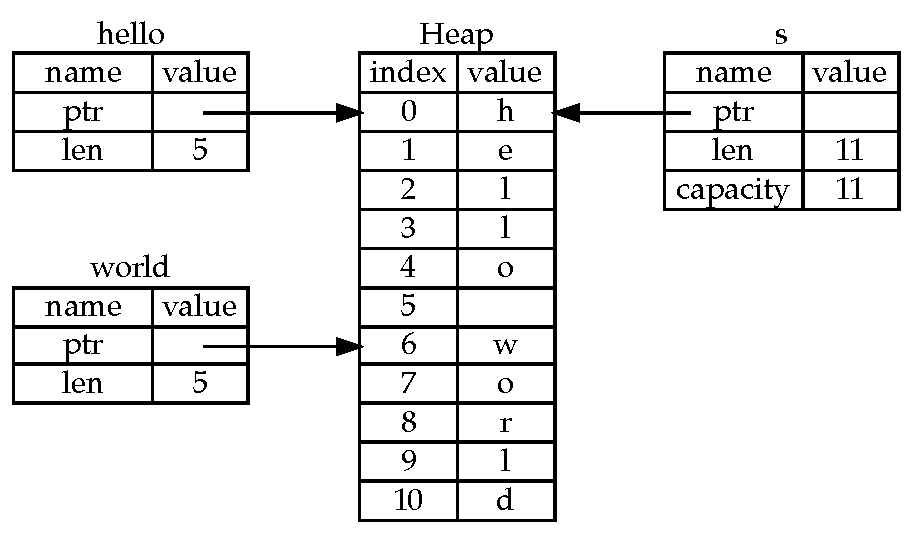
\includegraphics[scale=0.9]{Programmierung/Tabelle6.pdf}
    \caption{Diagramm eines String Slice}
    \label{fig:tabelle6}
\end{figure}

Dadurch entsteht eine Abhängigkeit, welche es Rust erlaubt, bereits beim Kompilieren festzustellen, ob String Slices auf einen gültigen Bereich im Speicher zeigen. So wird der Code weniger anfällig für Laufzeitfehler.

\begin{lstlisting}
    let s = "Hello, world!";
\end{lstlisting}

Der Typ von \verb"s" ist \verb"&str": Es ist ein String Slice, auf einen bestimmten Bereich einer Zeichenkette verweist. Deshalb sind String-Literale unveränderlich. \verb"&str" ist eine unveränderliche Referenz.

\subsubsection{Andere Slices}

String Slices sind speziell für Strings. Es gibt auch einen allgemeineren Slice-Typ für Arrays, bei dem wie bei String Slices auch hier Teile von Arrays referenziert werden können:

\begin{lstlisting}
    let a = [1, 2, 3, 4, 5];
    let slice = &a[1..3];
\end{lstlisting}

Der Typ von \verb"slice" ist \verb"&[i32]". Auch hier wird ein Pointer auf das erste Element sowie die Länge des Slice gespeichert.


\section{Modulsystem}

Dieses System von Rust ermöglicht die Erstellung von Modulen, welche mit Pfaden angesprochen werden können. Hiermit System können auch externe Pakete verwendet werden.

Module lassen den Code in Gruppen einteilen:

\begin{lstlisting}
    mod sound {
        mod instrument {
            mod string {
                fn guitar() {}
            }
        }
        mod voice {}
    }
\end{lstlisting}

Das Beispiel definiert das Modul \verb"sound" mit zwei inneren Modulen \verb"instrument" und \verb"voice" und ein Modul \verb"string" in \verb"instrument" mit der Funktion \verb"guitar". Der gesamte Modulbaum ist unter dem impliziten Modul namens \verb"crate" verwurzelt.

Diese Art von Baum erinnert an das Dateisystem eines Betriebssystems. Genau wie Verzeichnisse in einem Dateisystem kann im Code durch Module Code or\-ga\-ni\-siert werden. Eine weitere Ähnlichkeit zu Dateisystemen besteht darin, dass zum Verweisen auf ein Element dessen Pfad verwendet wird.

Es gibt zwei Arten von Pfaden:

\begin{itemize}
    \item Ein absoluter Pfad beginnend beim crate root mithilfe des crate-Namens oder dem Schlüsselwort \verb"crate".
    \item Ein relativer Pfad beginnend beim aktuellen Modul, er verwendet \verb"self", \verb"super" oder einen Bezeichner im aktuellen Modul.
\end{itemize}

Das Trennzeichen besteht aus zwei Doppelpunkten (\verb"::"). Folgende \verb"main"-Funktion könnte unter dem letzten Codebeispiel folgen:

\begin{lstlisting}
    fn main() {
        // absolute path
        crate::sound::instrument::string::guitar();

        // relative path
        sound::instrument::string::guitar();
    }
\end{lstlisting}

Dieser Code würde jedoch nicht kompilieren, da alle Elemente (Funktionen, Methoden, Strukturen, Enums und Konstanten) standardmäßig privat sind. Um ein Element öffentlich zu machen, kann das Schlüsselwort \verb"pub" verwendet werden.

Elemente ohne dem Schlüsselwort \verb"pub" sind privat, wenn der Modulbaum des aktuellen Moduls \glqq nach unten\grqq{} betrachtet wird. Elemente ohne \verb"pub" sind jedoch öffentlich, wenn sich diese auf der selben Ebene befinden oder der Baum \glqq nach oben\grqq{} betrachtet wird. In einem Dateisystem verhält es sich ähnlich: Ohne Berechtigung auf einen Ordner kann dieser nicht betrachtet werden. Auf einen zugänglichen Ordner können dessen Vorgängerverzeichnisse auch eingesehen werden.

Um die Funktion \verb"guitar" in der \verb"main"-Methode aufrufen zu können, müssen ei\-ni\-ge Module sowie die Funktion öffentlich gemacht werden:

\begin{lstlisting}
    mod sound {
        pub mod instrument {
            pub mod string {
                pub fn guitar() {}
            }
        }
        mod voice {}
    }
\end{lstlisting}

Relative Pfade können mit \verb"super" auch auf übergeordnete Module zugreifen, ähnlich wie bei einem Dateisystem mit \glqq\verb".."\grqq{}:

\begin{lstlisting}
    mod sound {
        pub mod instrument {
            pub fn clarinet() {
                super::breathe_in();
            }
        }
        fn breathe_in() {
            // Function body code
        }
    }
\end{lstlisting}

Häufig genutzte Pfade können mit dem Schlüsselwort \verb"use" gekürzt werden. Das ist vergleichbar mit einer Verknüpfung in einem Dateisystem. Es können absolute und relative Pfade benutzt werden.

\begin{lstlisting}
    use crate::sound::instrument;

    fn main() {
        instrument::clarinet();
    }
\end{lstlisting}

Externe Pakete können mit \verb"use"  eingebunden werden, dafür muss zunächst das Paket via Cargo.toml hinzugefügt werden:

\begin{lstlisting}
    [dependencies]
    rand = "0.6.5"
\end{lstlisting}

\noindent Im Code würde das so aussehen:

\begin{lstlisting}
    use rand::Rng;

    fn main() {
        let secret = rand::thread_rng().gen_range(1, 101);
    }
\end{lstlisting}

Der Quellcode kann mit dem Schlüsselwort \verb"mod" auf mehrere Dateien aufgeteilt werden, dabei ist der Name der Datei der Name des Moduls. Ordnerstrukturen können auch erstellt werden, dabei ist der Ordner selbst auch ein Modul, dessen Definition in der Datei \verb"mod.rs" definiert werden kann.

\vspace{0.5cm}

\noindent Datei \textbf{src/main.rs}

\begin{lstlisting}
    mod sound;

    fn main() {
        sound::instrument::clarinet();
    }
\end{lstlisting}

\vspace{0.5cm}

\noindent Datei \textbf{src/sound.rs}

\begin{lstlisting}
    pub mod instrument {
        pub fn clarinet() {
            // Function body
        }
    }
\end{lstlisting}


\section{Objektorientierung}

In der Programmiergemeinschaft herrscht kein Konsens darüber, welche Merkmale eine Sprache besitzen muss, um objektorientiert zu sein. Rust wird von vielen Programmierparadigmen beeinflusst, darunter auch von objektorientierter Programmierung (OOP). Objektorientierte Sprachen teilen üblicherweise drei Gemeinsamkeiten: Objekte, Kapselung und Vererbung.

Das Buch \textit{Design Patterns: Elements of Reusable Object-Oriented Software} von Erich Gamma, Richard Helm, Ralph Johnson und John Vlissides definiert OOP auf diese Weise:

\begin{quote}
    Object-oriented programs are made up of objects. An object packages both data and the procedures that operate on that data. The procedures are typically called methods or operations.
\end{quote}

Nach dieser Definition ist Rust objektorientiert. Strukturen und Enums enthalten Daten und \verb"impl" Blöcke stellen Methoden für diese bereit.

Eine Struktur in Rust in vergleichbar mit \verb"struct" in C oder C++. Rust kann diese Strukturen jedoch mit Methoden erweitern, sodass diese wie Klassen verwendet werden können.

Beispiel:

\begin{lstlisting}
    struct Employee {
        id: i32,
        age: i32,
        wage: f64,
    }
    
    impl Employee {
        fn birthday(&mut self) {
            self.age += 1;
        }
    }
    
    fn main() {
        let mut joe = Employee {
            id: 1,
            age: 32,
            wage: 48000.0,
        };
        joe.birthday();
    }
\end{lstlisting}

\subsection{Kapselung}

Ein weiterer Aspekt, welcher häufig mit OOP in Verbindung steht, ist die Idee der Kapselung. Das bedeutet, dass die Implementierung eines Objekts nicht für den Code verfügbar ist, der dieses Objekt verwendet.

Mit Modulen kann in Rust gekapselt werden, aber auch Strukturen und Enums sowie dessen Werte sind standardmäßig privat und können mit dem Schlüsselwort \verb"pub" öffentlich gemacht werden.

\begin{lstlisting}
    pub mod people {
        pub struct Employee {
            pub id: i32,  // public
            age: i32,     // private
            wage: f64,    // private
        }
    }
\end{lstlisting}

\subsection{Vererbung}

Vererbung ist ein Mechanismus, mit dem ein Objekt von der Definition eines anderen Objekts erben kann, wodurch die Daten und das Verhalten des über\-ge\-ord\-ne\-ten Objekts übernommen werden, ohne dass sie erneut definiert werden müssen.

Wenn eine Sprache Vererbung können muss, um eine objektorientierte Sprache zu sein, dann ist Rust keine. Es gibt keine Möglichkeit eine Struktur zu definieren, die Felder und Methodenimplementierungen der übergeordneten Struktur erbt.

Ein Beispiel der Vererbung in C++:

\begin{lstlisting}
    class Employee {
      public:
        string first_name, family_name;
        char middle_initial;
        Date hiring_date;
        short department;
        // ...
    };

    class Manager : public Employee {
        list<Employee *> group;
        short level;
        // ...
    };
\end{lstlisting}

Hier besitzt der Manager die gleichen Felder wie ein normaler Mitarbeiter zu\-sätz\-lich zu den eigenen Feldern.

\subsubsection{Warum verzichtet Rust auf Vererbung?}

In letzter Zeit ist die Vererbung als Entwurfslösung in vielen Programmiersprachen in Ungnade gefallen, da häufig die Gefahr besteht, dass mehr Code als erforderlich gemeinsam genutzt wird. Unterklassen sollten nicht immer alle Merkmale ihrer übergeordneten Klasse gemeinsam haben, dies geschieht jedoch mit Vererbung. Das kann das Design eines Programms weniger flexibel machen. Außerdem wird die Möglichkeit eingeführt, Methoden für Unterklassen aufzurufen, die keinen Sinn ergeben oder Fehler verursachen, da die Methoden nicht für die Unterklasse gelten. Darüber hinaus können in einigen Sprachen nur Unterklassen von einer Klasse erben, wodurch die Flexibilität der Sprache weiter einschränkt wird.

\subsection{Traits}

Ein \verb"trait" ist eine Sammlung von Methoden, die für einen unbekannten Typ definiert werden: \verb"Self". Sie können auf Methoden zugreifen, die im selben Trait definiert sind. Traits können für jeden Datentyp implementiert werden. \cite{RustExample}

\begin{lstlisting}
    pub trait Animal {
        fn noise(&self) -> &str;
    }
\end{lstlisting}

Dieses Trait definiert ein Tier, welches Geräusche von sich geben kann.

\begin{lstlisting}
    pub struct Sheep {
        pub name: String,
    }
    impl Animal for Sheep {
        fn noise(&self) -> &str {
            "baaaaaah"
        }
    }
\end{lstlisting}

Die Struktur \verb"Sheep" implementiert den Trait, sodass ein Schaf als Tier gesehen wird. Es können nun Funktionen geschrieben werden, die eine beliebige Tiere erwarten:

\begin{lstlisting}
    pub fn make_animal_speak(animal: &dyn Animal) {
        println!("Animal says {}.", animal.noise());
    }
\end{lstlisting}

Es können auch Listen von Trait-Objekten erstellt werden:

\begin{lstlisting}
    let mut animals: Vec<Box<dyn Animal>> = Vec::new();
    animals.push(Box::new(Sheep {}));
\end{lstlisting}

Das Schlüsselwort \verb"dyn" ist optional, dient aber zur besseren Unterscheidung zwi\-schen einem Trait (dyn) und einer Struktur (impl) und sollte daher immer verwendet werden.

Der Typ \verb"Box" ist ein Pointer mit einer festen Speichergröße, mit dem Werte auf dem Heap gespeichert werden können. Er wird benötigt, da zur Kompilierzeit die Größe des Datentyps noch nicht bekannt ist.

\subsubsection{Trait-Objekte benutzen dynamische Bindung (dynamic dispatch)}\label{dynamicdispatch}

Wenn Trait-Objekte für Funktionen verwendet werden, muss Rust die dynamische Bindung benutzen. Der Compiler kennt nicht alle Typen, die möglicherweise für den Code verwendet werden, sodass er nicht weiß, welche Methode für welchen Typ der Aufruf implementiert ist. Stattdessen verwendet Rust zur Laufzeit Zeiger im Trait-Objekt, um zu ermitteln, welche Methode aufgerufen werden soll. Wenn diese Suche ausgeführt wird, fallen Laufzeitkosten an, die beim statischen Binden (static dispatch) nicht auftreten würden. Die dynamische Bindung verhindert auch, dass der Compiler den Code einer Methode direkt an die entsprechende Stelle kopiert, wodurch Optimierungen verhindert werden können. Jedoch erhält man durch Traits zusätzliche Flexibilität im Code, es ist also ein Kompromiss.


\section{Generische Programmierung}

Ähnlich wie in C++ (Templates) gibt es auch in Rust die Möglichkeit, Typen als Argumente zu übergeben, ohne Informationen zu verlieren. Das bedeutet: Es können Funktionssignaturen oder Strukturen erstellt werden für Elemente, die viele verschiedene konkrete Datentypen verwenden können.

Beispiel in Rust:

\begin{lstlisting}
    #[derive(Debug)]
    struct Point<T> {
        x: T,
        y: T,
    }
    
    impl<T> Point<T> {
        fn new(x: T, y: T) -> Point<T> {
            Point { x: x, y: y }
        }
    }
    
    fn main() {
        let p1 = Point::new(1, 2);
        let p2 = Point::new(1.0, 2.0);
    }
\end{lstlisting}

Die Klasse \verb"Point" beinhaltet zwei Werte deren Typen erst bei der Erstellung des Objekts bekannt werden. Beide Variablen \verb"x" und \verb"y" haben den gleichen Typ \verb"T". Die Variable \verb"p1" ist ein \verb"Point<i32>" und \verb"p2" ein \verb"Point<f64>".

Es können auch Typen verwendet werden, die bestimmte Traits implementieren müssen:

\begin{lstlisting}
    fn animal_noise<T: Animal>(animal: T) {
        println!("This animal makes {}.", animal.noise());
    }
\end{lstlisting}

C++ und Rust implementieren Generics so, dass Code mit generischen Typen nicht langsamer läuft als mit konkreten Typen. Rust erreicht dies dadurch, dass beim Kompilieren generischer Code in spezifischen Code umgewandelt wird und die konkreten Typen eingetragen werden. Dieser Prozess wird Monomorphisierung genannt.


\section{Unit-Tests}\label{chap:unittests}

Rust wurde mit einem hohen Maß an Sorge um die Richtigkeit von Programmen entworfen. Richtigkeit ist jedoch nicht leicht nachzuweisen. Das Typensystem von Rust kann nicht jede Art von Fehler verhindern, daher bietet Rust Unterstützung für das Schreiben automatisierten Softwaretests.

In C oder C++ gibt es Frameworks, welche von Dritten angeboten werden. Ein Beispiel ist Google Test\footnote{https://github.com/google/googletest}.

Für Unit-Tests in Rust wird nach Konvention in jeder Datei ein Modul mit dem Namen \verb"tests" erstellt mit der Annotation \verb"#[cfg(test)]". Hier werden Testfunktionen definiert mit der Annotation \verb"#[test]". Diese Unit-Tests werden mit dem Befehl \verb"cargo test" gestartet.

\begin{lstlisting}
    #[cfg(test)]
    mod tests {
        #[test]
        fn it_works() {
            assert_eq!(2 + 2, 4);       // assert equal
            assert_ne!(2 + 2, 22);      // assert not equal
        }
    }
\end{lstlisting}

Folgende Makros sind hilfreich bei der Erstellung von Tests:

\begin{itemize}
    \item \verb"assert!(a)": Prüft einen Boolean-Wert; Panik bei \verb"false".
    \item \verb"assert_eq!(a,b)": Vergleicht zwei Werte; Panik bei unterschiedlichen Werten.
    \item \verb"assert_ne!(a,b)": Wie \verb"assert_eq!"; Panik bei gleichen Werten.
    \item \verb"panic!()": Generiert Panik und der Test schlägt fehl.
\end{itemize}

Diese Makros können zusätzlich einen Text für mehr Informationen ausgeben:

\begin{lstlisting}
    assert_eq!(a, b, "Testing equality of {} and {}", a, b);
\end{lstlisting}


\section{Error Handling}

\subsection{Fehler mit \texttt{panic!}}

Wenn im Code ein Fehler auftritt, kann das Makro \verb"panic!" benutzt werden. Im letzten Kapitel wurde wurde es bereits erläutert, um Tests fehlschlagen zu lassen. Beim Aufruf dieses Makros gibt das Programm eine Fehlermeldung aus, räumt den Stack auf und beendet sich.

Wenn also eine Panik auftritt, wird das Programm standardmäßig beendet. Das bedeutet, dass Rust den Stack zurücksetzt und die Daten aller Funktionen bereinigt, auf die er stößt. Aber das Zurückgehen des Stacks und Aufräumen ist eine Menge Arbeit. Die Alternative ist, sofort abzubrechen, wodurch das Programm ohne Be\-rei\-ni\-gung beendet wird und der vom Programm verwendete Speicher vom Be\-triebs\-sys\-tem bereinigt werden muss. Wenn in einem Projekt die resultierende Binärdatei so klein wie möglich gestaltet werden soll, kann bei einer Panik vom \glqq Abwickeln\grqq{} auf \glqq Abbrechen\grqq{} gewechselt werden, indem in der Cargo.toml \verb"panic = 'abort'" in die entsprechenden Abschnitte geschrieben wird:

\begin{lstlisting}
    [profile.release]
    panic = 'abort'
\end{lstlisting}

Eine Panik kann beispielsweise auch ausgelöst werden, wenn im Code auf ein Element eines Vektors zugegriffen wird, welches nicht innerhalb des Bereichs liegt:

\begin{lstlisting}
    fn main() {
        let v = vec![1, 2, 3];
        v[99];
    }
\end{lstlisting}

In diesem Codebeispiel wird auf das 100. Element des Listenelements \verb"v" zugegriffen. Dadurch entsteht folgende Fehlermeldung:

\begin{lstlisting}
    thread 'main' panicked at 'index out of bounds: the len
    is 3 but the index is 99'
\end{lstlisting}

In C und C++ würden bei Arrays keine Fehlermeldungen erscheinen und es würde ein Zahlenwert ausgegeben werden, der davon abhängig ist, was in diesem Moment im Speicher steht. In C++ können jedoch alternativ Listen erstellt werden (z. B. \verb"vector<int>"), die zur Laufzeit überprüfen können, ob die Zugriffe innerhalb des Bereichs der Liste stattfinden.

\subsection{Fehler mit \texttt{Result}}

Viele Fehler sind nicht schwerwiegend genug, um ein vollständiges Anhalten des Programms zu erfordern. Wenn beispielsweise eine nicht existierende Datei geöffnet werden soll, könnte diese erstellt werden, anstatt das Programm zu beenden.

Das Enum \verb"Result" ist in der Standardbibliothek definiert:

\begin{lstlisting}
    enum Result<T, E> {
        Ok(T),
        Err(E),
    }
\end{lstlisting}

Bei \verb"T" und \verb"E" handelt es sich um generische Typparameter. Dabei stellt \verb"T" den Typ des Werts dar, der in einem Erfolgsfall innerhalb der \verb"Ok" Variante zurückgegeben wird und \verb"E" stellt die Art des Fehlers dar, der in einem Fehlerfall innerhalb der \verb"Err" Variante zurückgegeben wird.

So wird eine Funktion aufgerufen, die ein \verb"Result" zurückgibt, weil sie fehlschlagen könnte.

\begin{lstlisting}
    use std::fs::File;
    fn main() {
        let f = File::open("hello.txt");
    }
\end{lstlisting}

In der Standardbibliothek steht beschrieben, welchen Typ die Funktion zu\-rück\-gibt, \verb"f" ist vom Typ \verb"Result<File, Error>". Mithilfe des \verb"match"-Statements kann getestet werden, ob die Funktion korrekt ausgeführt wurde oder, bei Misserfolg, welche Art von Fehler entstanden ist.

\begin{lstlisting}
    use std::fs::File;
    use std::io::ErrorKind;

    let f = match f {
        Ok(file) => file,
        Err(error) => match error.kind() {
            ErrorKind::NotFound => /*TODO: create file*/
                                   panic!(),
            other_error => panic!("could not open: {:?}",
                           other_error),
        }
    };
\end{lstlisting}

Der Aufruf \verb"error.kind()" gibt ein Enum \verb"ErrorKind" zurück, womit auf verschiedene Fehlerszenarien reagiert werden kann.

\subsubsection{Fehler weitergeben}

Beim Schreiben einer Funktion, welche möglicherweise einen Fehler aufruft, kann der Fehler an den aufrufenden Code zurückgegeben werden, anstatt den Fehler in dieser Funktion zu behandeln. Somit wird dem aufrufendem Code mehr Kontrolle gegeben. Anstelle des Aufrufs von \verb"panic!" wird ein \verb"return"-Statement verwendet. Alternativ kann der \verb"?"-Operator verwendet werden.

\subsection{\texttt{?}-Operator}

Codebeispiel:

\begin{lstlisting}
    use std::io;
    use std::Read;
    use std::fs::File;

    fn read_username() -> Result<String, io::Error> {
        let mut f = File::open("hello.txt")?;
        let mut s = String::new();
        f.read_to_string(&mut s)?;
        Ok(s)
    }
\end{lstlisting}

Wird ein \verb"?" hinter ein \verb"Result" geschrieben und der Wert ist ein \verb"Ok", wird der Wert innerhalb des \verb"Ok" von diesem Ausdruck zurückgegeben und die Funktion wird fortgesetzt. Wenn es sich bei dem Wert um einen Fehler handelt, wird der Fehler von der gesamten Funktion zurückgegeben, als ob das Schlüsselwort \verb"return" verwendet wurde. Dieser Operator kann nur innerhalb von Funktionen verwendet werden, welche ein \verb"Result" als Rückgabetyp haben. Dadurch wird die Implementierung vereinfacht und die Lesbarkeit des Codes verbessert.

\subsection{Error Handling in C und C++}

In C gibt es keine direkte Unterstützung für die Fehlerbehandlung, es gibt aber Möglichkeiten, wie sie dennoch durchgeführt werden kann. Viele C-Funk\-ti\-ons\-auf\-ru\-fe geben im Fehlerfall \verb"-1" oder \verb"NULL" zurück, sodass mit einer \verb"if"-Anweisung entsprechend reagiert werden kann. Die globale Variable \verb"errno" kann zusätzlich zur Unterscheidung verwendet werden.

C++ bietet einige hilfreiche Features. Die \verb"throw"-Anweisung kann Ausnahmen an einen Handler übergeben, ähnlich wie es beispielsweise in Java üblich ist. Zusätzlich können statische Assertionen benutzt werden, um zur Kompilierzeit bestimmte Eigenschaften sicherzustellen.


\section{Dokumentieren mit rustdoc}

Ein wichtiger Bestandteil bei der Programmierung in Rust ist das Erstellen von Dokumentationen. Das Tool \verb"rustdoc" ist vergleichbar mit \verb"javadoc" für Java. Es können im Code spezielle Kommentare geschrieben werden und daraus wird eine Dokumentation mit HTML, CSS und JavaScript erstellt.

\subsection{Grundlegende Verwendung}

Folgendes Beispiel zeigt die grundsätzliche Verwendung der Kommentare, sie werden mit drei Schrägstrichen gekennzeichnet. Alternativ kann die Annotation \verb"#[doc]" verwendet werden.

\begin{lstlisting}
    /// foo is a function
    pub fn foo() {}
\end{lstlisting}

Alternative Schreibweise:

\begin{lstlisting}
    #[doc = "foo is a function"]
    pub fn foo() {}
\end{lstlisting}

Es können in den Kommentarzeilen Elemente aus Markdown verwendet werden, um z. B. Überschriften oder Listenaufzählungen zu erstellen.

Die Dokumentation kann auf der Kommandozeile mit einem Cargo-Befehl ge\-ne\-riert werden:

\begin{lstlisting}
    $ cargo doc
\end{lstlisting}

Nach dem Kompilieren ist die \verb"index.html" anschließend zu finden unter dem Pfad \texttt{./target/doc/[crate-name]/index.html}.

\subsection{Dokumentationstests}

Rust erlaubt die Ausführung von Tests innerhalb der Codebeispiele in der Dokumentation. Codebeispiele werden mit drei Akzentzeichen (\verb"```") am Anfang und am Ende des Codes gekennzeichnet.

\begin{lstlisting}
    /// # Examples
    /// ```
    /// let x = 5;
    /// assert_eq!(x, 5);
    /// ```
\end{lstlisting}

Bei einem Aufruf von \verb"cargo test" wird dieser Code ausgeführt, der Code muss also kompilierbar sein. Alle \verb"assert"-Funktionen können hier verwendet werden.

Es gibt ein paar nützliche Annotationen, mit denen Dokumentationstests zu\-sätz\-lich angepasst werden können.

\begin{itemize}
    \item \verb"ignore": Der Code wird von Rust ignoriert.
\begin{lstlisting}
    /// ```ignore
    /// fn foo() {
    /// ```
\end{lstlisting}
\item \verb"should_panic": Der Test sollte eine Panik auslösen.
\begin{lstlisting}
    /// ```should_panic
    /// assert!(false);
    /// ```
\end{lstlisting}
\item \verb"no_run": Der Code wird kompiliert aber nicht ausgeführt.
\begin{lstlisting}
    /// ```no_run
    /// loop {
    ///     println!("Hello, world");
    /// }
    /// ```
\end{lstlisting}
\item \verb"compile_fail": Der Code soll beim Kompilieren einen Fehler ausgeben.
\begin{lstlisting}
    /// ```compile_fail
    /// let x = 5;
    /// x += 2; // shouldn't compile!
    /// ```
\end{lstlisting}
\end{itemize}


\section{WebAssembly}

WebAssembly ist eine Technologie mit der performante Webanwendungen programmiert werden können. Es handelt sich dabei um einen Binärcode, der aus verschiedenen Programmiersprachen generiert werden kann, darunter C, C++ und Rust. Rust bietet Programmierern eine Low-Level-Kontrolle und zuverlässige Leistung. Es ist frei von Pausen durch Garbage-Collection aus JavaScript und Programmierer haben Kontrolle über Pointer, Monomorphisierungen und Speicherlayout.

Zum Erstellen von WebAssembly Projekten in Rust werden die Cargo-Pakete \verb"wasm-pack", \verb"cargo-generate" und der Paketmanager für JavaScript NPM benötigt. \cite{RustWebAssembly}

\subsection{Beispielprojekt in Rust anlegen}

Rust bietet eine Vorlage auf Github an, die mit Cargo heruntergeladen werden kann.

\begin{lstlisting}
    $ cargo generate --git https://github.com/rustwasm/wasm-
      pack-template
\end{lstlisting}

Dadurch entsteht ein Rustprojekt mit einer Cargo.toml sowie zwei Quellcodedateien \verb"lib.rs" und \verb"utils.rs" im \verb"src"-Ordner.

Die Cargo.toml ist vorkonfiguriert für die Erstellung von \verb".wasm" Bibliotheken. Die Quelldateien definieren ein Beispielprogramm, welches die Funktion \verb"alert" aus JavaScript in Rust importiert und eine Funktion \verb"greet" von Rust exportiert.

Um das Projekt zu bauen, müssen die Rust-Quelldateien in \verb".wasm" Binärdateien kompiliert und eine JavaScript API generiert werden um das generierte WebAssembly zu benutzen. Dies geschieht mit einem Befehl:

\begin{lstlisting}
    $ wasm-pack build
\end{lstlisting}

Die generierten Dateien werden im Ordner \verb"pkg" gespeichert. Dort befindet sich die \verb".wasm"-Datei und eine \verb".js"-Datei, welche die WebAssembly-Daten importiert und die in Rust programmierte \verb"greet" Funktion als JavaScript-Funktion verpackt.

\subsubsection{Webseite}

Um den Code auf einer Webseite zu benutzen, kann mit Node.js die Projektvorlage \verb"create-wasm-app" verwendet werden:

\begin{lstlisting}
    $ npm init wasm-app www
\end{lstlisting}

Nun müssen die Abhängigkeiten installiert werden, folgender Befehl muss im Unterordner \verb"./www" ausgeführt werden:

\begin{lstlisting}
    $ npm install
\end{lstlisting}

In der Datei \verb"./www/package.json" muss bei den Abhängigkeiten das Projekt hinzugefügt werden:

\begin{lstlisting}
    "devDependencies": {
        "name-of-project": "file:../pkg",
        // ...
    }
\end{lstlisting}

Im JavaScript-Code kann nun \verb"name-of-project" importiert werden. Jetzt muss die neue Abhängigkeit installiert werden und der Webserver kann gestartet werden. Im Verzeichnis \verb"./www":

\begin{lstlisting}
    $ npm install
    $ npm run start
\end{lstlisting}

Im Browser kann unter der URL http://localhost:8080/ die Webseite aufgerufen werden.
